\documentclass[11pt,twocolumn]{article}
\renewcommand{\thesection}{\Roman{section}}
\renewcommand{\thesubsection}{\thesection.\Alph{subsection}}
\usepackage[utf8x]{inputenc}
\usepackage{ifpdf}
\usepackage{multicol}
\usepackage{placeins}
\usepackage{qtree}
\usepackage{placeins}
\usepackage{fancyhdr}
\usepackage{cite}
%\renewcommand{\cite}{\textcolor{red}}
\usepackage{url}
\usepackage[english]{babel}


\ifpdf 
    \usepackage[pdftex]{graphicx}   % to include graphics
    \pdfcompresslevel=9 
    \usepackage[pdftex,     % sets up hyperref to use pdftex driver
            plainpages=false,   % allows page i and 1 to exist in the same document
            breaklinks=true,    % link texts can be broken at the end of line
            colorlinks=true,
            linkcolor=blue,
            citecolor=blue,
            pdftitle=My Document
            pdfauthor=My Good Self
           ]{hyperref} 
    \usepackage{thumbpdf}
\else 
    \usepackage{graphicx}       % to include graphics
\usepackage{color}
\usepackage[colorlinks=true,
        linkcolor=blue, citecolor=blue]{hyperref}

\fi 
\pagestyle{fancy}
\fancyhf{}
\lhead{}
\rhead{}
\cfoot{\thepage}
\onecolumn
\title{\textbf{Lab Course: Hardware/Software Co-Design with a LEGO Car\\[3ex]}
\normalsize{%Received 10/30/2015  22:20:00 Revised 10/30/2015  22:20:00 
\textbf{Abdallah Attawia, Moritz Dötterl, Heiko, Berkay} \\
%Matriculation Number: 03664889} \\[3ex]
Technische Universität München, Garching, Department of Informatics \\
Boltzmannstr. 3, 85748 Garching, Germany  \\
%e-mail address: abdallah.attawia@tum.de \\[3ex] 
\begin{flushleft}
This document explains the work done on a lego car to detect and follow a line autonomously. Connection and communication between the hardware parts is explained. Furthermore, collision avoidance and line detection algorithms are thoroughly described.    
\end{flushleft}
}}

\twocolumn

\begin{document}
\date{}
\maketitle
\noindent
\section{Introduction}
An autonomous car is one that can drive from point A to B independently without any human input. It can accelerate, brake and steer itself as well as sense the environment and navigate to avoid crashing. The development of autonomous vehicles is rapidly growing and a lot of big and small companies are working towards making autonomous driving a reality.\\
In this project a small scaled model, a lego car, along with some cheap components are used to test a real autonomous driving function, i.e. following a line on the street. This documentation starts with a brief explanation of the different hardware components. Then the cabling and communication between the components is described. Lastly, the collision avoidance technique and and the line detection and following are explained. The code, attached to this report, carries out the functions explained here and is clearly documented.
\section{Hardware Parts} 
The hardware components used are two controllers, the DEO-Nano and the Raspberry Pi, two types of actuators, namely speed motors and servo motors, as well as two types of sensors, which are the ultrasound sensors and the USB-camera.
\subsection{DEO-Nano} 
The DE0-Nano board is a compact-sized FPGA based development platform manufactured by terasIC. Its heart is a Cyclone IV FPGA from Altera. Furthermore it features on board memory, LEDs, Buttons, and most importantly three GPIO headers. On this FPGA we flashed the provided Nios-II image. This is an image of an adaptable processor allowing for custom specializations such as multiple hardware UART handlers. Now it is possible to wright code for this processor in C using the hardware you &desire, without any trade off.
\subsection{Raspberry Pi}
For this project the newly released Raspberry Pi 3 is used. Raspberry Pi is a small-sized one board computer. In this work it is used to connect the camera with the Nano-board and to run the line following code.\\
First, the computer is connected to the Raspberry Pi using Secure Schell (SSH) and the Raspbian Operating System is installed. Then the camera is connected using one of the USB ports and OpenCV is installed to run the line following code. Finally uart communication is enabled to connect the Raspberry Pi with the Nano-board. In Raspberry Pi 3 you need to disable Bluetooth in order for uart communication to work. To disable onboard Pi3 Bluetooth and restore uart over GPIOs 14 and 15, modify the file "/boot/config.txt":
\begin{itemize}
\item {sudo nano /boot/config.txt}
\item {Add this to the end of the file "dtoverlay=pi3-disable-bt"}
\end{itemize}
\subsection{Actuators}
\begin{itemize}
	\item{Speed motors}
	\item{Servo motor}
\end{itemize}
\subsection{Sensors} 
\begin{itemize}
	\item{Ultrasound sensor} \\
	The ultrasound sensor measures the distance from any detected object within its range. As shown in Figure \ref{ultrasound} the ultrasound sensors detects objects by sending out ultrasound waves and receiving an echo, if an object is detected. The sensor measures the time of flight between transmitting and receiving the signal and calculates the distance according to the following formula (\ref{dis}).
	
\begin{equation}
\centering
L = \frac{340(m/s)x\bigtriangleup t(s)}{2}
\label{dis}
\end{equation}

\begin{figure}[h]
\centering
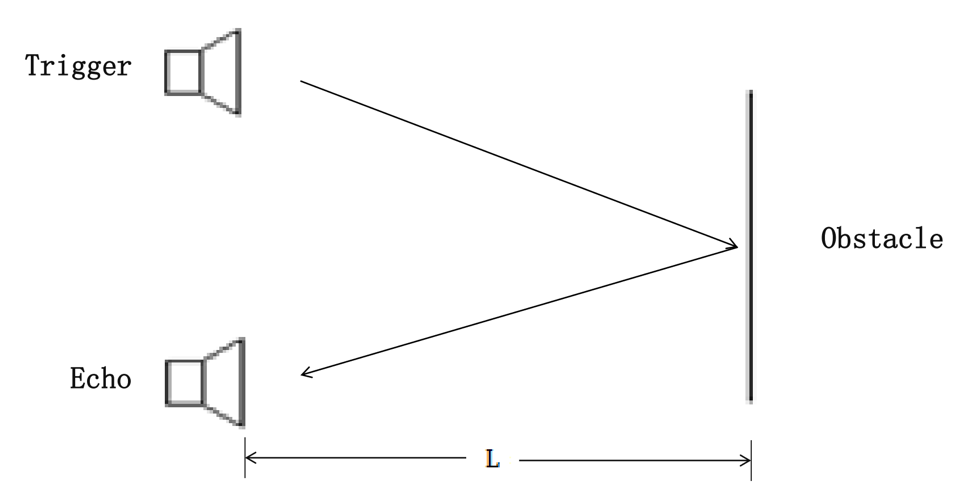
\includegraphics[width=0.5\textwidth]{ultrasound.png}
\caption{Theory of operation of the ultrasound sensor}
\label{ultrasound}
\end{figure}

In this course, the KS103 ultrasound sensor is used. It has a range up to 11m which can be specified by sending a command from the Nano-board. This sensor can operate using two digital communication protocols; I2C and Uart. It has an accuracy between $1mm$ and $10mm$\\
In order for the ultrasound sensor to operate, it is first initialized and set to the desired range. Like the raspberry pi, it communicates with the Nano-board using uart communication, which has to be initialized as well. The Nano-board then sends a command to the sensor to send the data using uat. The Nano-board finally receives date from the sensor. The data read from the sensor is multiplied times 170 to get the distance from detected objects in micrometer.  
	\item{USB Camera}
\end{itemize}

\section{Cabling}

\section{Communication}

\section{Collision Avoidance}
In order to avoid collisions, an algorithm based on the idea of the adaptive cruise control is implemented. Adaptive cruise control is a cruise control function that allows the vehicle to adapt its speed according to the traffic and to maintain a safe distance from the vehicles ahead.\\
In real cars, a long range radar sensor is used to detect the cars, here we use an ultrasound sensor to measure the distance from the vehicles ahead. The following algorithm is implemented to avoid the collision with other cars or objects and to adapt the speed to the surrounding traffic.
\begin{itemize}
	\item if distance from ultrasound sensor $\leq$ a minimum set distance ($distance_{min}$)\\
	-car stops
	\item if distance from ultrasound sensor $\geq$ a maximum set distance ($distance_{max}$)\\
	 -drive with maximum speed
	\item else (distance lies within $distance_{min}$ and $distance_{max}$)\\
	 -adapt speed according to distance:
	 \begin{equation}
	 Current Speed = Maximum Speed * \frac{distance}{distance_{max}}
	 \end{equation}
\end{itemize}

The speed of the car is set according to the aforementioned algorithm, where the current speed is the duty cycle that is assigned to the speed motors.
\section{Image processing for line detection and following}
\subsection{Code}
\subsection{Optimization}

\section{Conclusion}
To conclude, the car followed a closed track without getting out of line in both directions. The maximum set speed was about 85\% of the maximum possible speed. If the camera had had a wider view, the full motor speed could had been reached.

\section*{Acknowledgments}


\begin{small}
\bibliography{mybib}
\bibliographystyle{ieeetr}
\end{small}




\end{document}

% I removed the typos and 
% I described the general hardware implementations in the opening statement of the review and stated the most significant differences. Also, I removed the unnecessary hardware descriptions in the following subsections.
% I started each subsection with a brief explanation of the control methods then described them briefly using an example in one of the systems.
% I tried to make the control methods as understandable as possible and to explain the unclear terminologies.